
\typeout{}\typeout{If latex fails to find aiaa-tc, read the README file!}
%


\documentclass[]{aiaa-tc}% insert '[draft]' option to show overfull boxes

\usepackage{mathptmx}         %CHANGE FONT TO TIMES NEW ROMAN

\usepackage{amsmath}          % for formula writing (i.e. 'split', etc)
\usepackage{rotate}           %rotate/mirror images
\usepackage{cancel}           %draw lines through math to show "goes to zero"
\usepackage{xfrac}            %allows slated and side fractions
\usepackage{subcaption}       %allows captioning individual subfigures
\usepackage{multicol}         %enable environment with multiple columns
\usepackage[mode=buildnew]{standalone}% requires -shell-escape
  % compile with `pdflatex -shell-escape main` or `xelatex  -shell-escape main`



\usepackage{tikz}             %for creating vector graphics diagrams
\usetikzlibrary{backgrounds}  %put backgrounds behind tikz figures
\usetikzlibrary{calc}         %perform calculations within $$
\usetikzlibrary{positioning}  %position tikz elements using "right of, etc"
\usetikzlibrary{angles}       %label angles between lines with arcs
\usetikzlibrary{quotes}       %Put angle label in quotes
\usetikzlibrary{patterns}     %Patterns to fill shapes with







\usepackage{caption}          %caption graphics ('\captionof')
\usepackage{framed}           %allows shaded text
\usepackage[T1]{fontenc}      %allows escaping specific charaters like '_'


%%%%%%%%%%%%%%%%%%%%%%%%%%%%%%%%%%%%%%%%%%%%%%%%%%%%%%
%HYPERLINKS
\usepackage{hyperref}     %insert hyperlines with '\url' or '\href'
\newcommand\linkcolor{blue} %variable to color url text

%%%%%%%%%%%%%%%%%%%%%%%%%%%%%%%%%%%%%%%%%%%%%%%
%CODE LISTING SYNTAX COLORING
\usepackage{color}     %make custom colors for syntax coloring
\usepackage{listings}  %allows code listings
\usepackage{textcomp}  %allows apostrophes to be straight (unidirectional)
% \usepackage{framed}
% \usepackage{caption}
\usepackage{bm}
\usepackage{tcolorbox}        %use for code listing color definitions
\tcbuselibrary{listings}      %allow color defenitions in code listings
\tcbuselibrary{breakable}     %allow tccolorboxes across page breaks
\tcbuselibrary{most}     %allow tccolorboxes across page breaks

\captionsetup[lstlisting]{font={small,tt}} %setup caption style

%Custom Colors
\definecolor{mygreen}{rgb}{0,0.6,0}
\definecolor{mygray}{rgb}{0.5,0.5,0.5}
\definecolor{mymauve}{rgb}{0.58,0,0.82}

\definecolor{sublimeblack}{HTML}{272822}
\definecolor{sublimered}{HTML}{F92672}
\definecolor{sublimeblue}{HTML}{66D9EF}
\definecolor{sublimeyellow}{HTML}{E6DB74}
\definecolor{sublimegrey}{HTML}{75715E}
\definecolor{sublimegreen}{HTML}{66CC33}
\definecolor{sublimeorange}{HTML}{FD971F}
\definecolor{sublimepurple}{HTML}{AE81FF}


%White or Black background toggle
\newcommand\whiteback{0}
\ifnum\whiteback=1%
  %White Background
  \newcommand\backclr{white}
  \newcommand\txtclr{\color{black}}
  \newcommand\txtupclr{black} %same as text color, used elsewhere
  \newcommand\comclr{\color{sublimegrey}}
  % \newcommand\comclr{\color{mygreen}}
  \newcommand\keyclr{\color{sublimeblue}}
  % \newcommand\keyclr{\color{blue}}
  \newcommand\ndkeyclr{\color{sublimered}}
  \newcommand\strclr{\color{mygreen}}
  % \newcommand\strclr{\color{sublimeyellow}}
  \newcommand\frameon{single} %single-frame box around code

\else
  %Black Background (like SublimeText)
  \newcommand\backclr{sublimeblack}
  \newcommand\txtclr{\color{white}} %text color
  \newcommand\txtupclr{white} %same as text color, used elsewhere
  \newcommand\comclr{\color{sublimegrey}}
  \newcommand\keyclr{\color{sublimeblue}}
  \newcommand\ndkeyclr{\color{sublimered}}
  \newcommand\strclr{\color{sublimeyellow}}
  \newcommand\frameon{false} %no frame for black background
\fi


%Listing Style
% \newcommand\lstfontsize{\scriptsize}
\newcommand\lstfontsize{\small}
\lstdefinestyle{mystyle}{%
  % backgroundcolor=\backclr,   % choose the background color; you must add \usepackage{color} or \usepackage{xcolor}
  basicstyle=\ttfamily\txtclr\lstfontsize, % the SIZE OF THE FONTS that are used for the code
  breakatwhitespace=false,         % sets if automatic breaks should only happen at whitespace
  % breaklines=true,                 % sets automatic line breaking
  captionpos=b,                    % sets the caption-position to bottom
  commentstyle=\comclr,            % comment color
  deletekeywords={...},            % if you want to delete keywords from the given language
  escapeinside={\%*}{*)},          % if you want to add LaTeX within your code
  extendedchars=true,              % lets you use non-ASCII characters; for 8-bits encodings only, does not work with UTF-8
  frame=\frameon,                  % adds a frame around the code
  keepspaces=true,                 % keeps spaces in text, useful for keeping indentation of code (possibly needs columns=flexible)
  columns=flexible,
  otherkeywords={zip,enumerate,True,False,None,...},  %add words to be highlighted
  keywordstyle=\keyclr,            % keyword (e.g. 'print') color
  language=Python,                 % the language of the code
  upquote=true,                    % make apostrophes straight (unidirectional)
  alsoletter={<>=-+*/!},            % to avoid coloring operators when they're not
  ndkeywords={=,+,-,*,**,/,+=,*=,-=,/=,<=,>=,==,!=,<,>,... },  % operator keywords
  ndkeywordstyle=\ndkeyclr,         % style of operator keywords
  numbers=left,                    % where to put the line-numbers; possible values are (none, left, right)
  numbersep=5pt,                   % how far the line-numbers are from the code
  numberstyle=\tiny\color{mygray}, % line-number style: size, color
  rulecolor=\color{black},         % if not set, the frame-color may be changed on line-breaks within not-black text (e.g. comments (green here))
  showspaces=false,                % show spaces everywhere adding particular underscores; it overrides 'showstringspaces'
  showstringspaces=false,          % underline spaces within strings only
  showtabs=false,                  % show tabs within strings adding particular underscores
  stepnumber=1,                    % the step between two line-numbers. If it's 1, each line will be numbered
  stringstyle=\strclr,             % string color
  tabsize=4,                       % sets default tabsize
}


%Function that calls listing of specific file with custom coloring
  %first input is filename to list
  %next two inputs are start and end line numbers
    %(use 0 and large number for all lines)
\newcommand\mylisting[3]{
  \tcbinputlisting{
        listing file=#1,
        breakable,
        nobeforeafter,
        arc=0pt,
        top=0mm,
        bottom=0mm,
        left=0mm,
        right=0mm,
        boxrule=0pt,
        colback=\backclr, %background color (continue accross page breaks)
        colupper=\txtupclr, %basic text color (continue accross page breaks)
        listing only,
        listing options={
                            style=mystyle,            %use custom style
                            firstline=#2,lastline=#3, %lines of code to use
                            firstnumber=#2,           %same numbering as script
                        },
        % hbox %Turning this on prevents page breaks
      }
}







  \title{MAE 210B Turbulence -- Term Project \\ RANS Turbulence Modeling Sensitivity of Parachute-like Bodies}


\author{
  Logan D. Halstrom \\
  {\normalsize\itshape Graduate Student} \\
  {\normalsize\itshape Department of Mechanical and Aerospace Engineering} \\
  {\normalsize\itshape University of California, Davis, CA 95616}
       }


 % Define commands to assure consistent treatment throughout document
 \newcommand{\eqnref}[1]{(\ref{#1})}
 \newcommand{\class}[1]{\texttt{#1}}
 \newcommand{\package}[1]{\texttt{#1}}
 \newcommand{\file}[1]{\texttt{#1}}
 \newcommand{\BibTeX}{\textsc{Bib}\TeX}



%%%%%%%%%%%%%%%%%%%%%%%%%%%%%%%%%%%%%%%%%%%%%%%%%%%%%%%%%%%%%%%%%%%%%%%%
\begin{document}

\maketitle


% % %%%%%%%%%%%%%%%%%%%%%%%%%%%%%%%%%%%%%%%%%%%%%%%%%%%%%%%%%%%%%%%%%%%%%%%%
% \begin{abstract}

% Abstract about lit study

% \end{abstract}





% %%%%%%%%%%%%%%%%%%%%%%%%%%%%%%%%%%%%%%%%%%%%%%%%%%%%%%%%%%%%%%%%%%%%%%%%
% \section*{Nomenclature}

% \begin{multicols}{2}

% \begin{tabbing}
%   XXX \= \kill% this line sets tab stop
%   $0$                 \> Subscript for quiescent parameters \\
%   $e$                 \> Subscript for emission parameters \\
%   $L$                 \> Subscript for loading parameters \\
%   $t$                 \> Time \\
%   $\tau$              \> Retarded time \\
%   $ret$               \> Evaluated at retarded time \\
%   $\hat{n}$           \> Unit surface normal vector \\
%   $\vec{r}$           \> Radial direction vector \\
%   $\hat{r}$           \> Radial unit vector \\
%   $r$                 \> Magnitude of radial vector $|\vec{r}|$ \\
%   $\theta$            \> Angle between $\hat{n}$ and $\hat{r}$ \\
%   $f$                 \> Function of surfaces within a fluid space \\
%   $\vec{V}$           \> General velocity vector \\
%   $V_r$               \> Velocity component in radial direction \\
%   $V_n$               \> Velocity component in surface normal direction \\
%   $M$                 \> Mach number \\
%   $c$                 \> Speed of Sound\\
%   $\overline{\rho}$   \> Mean density \\
%   $p$                 \> Pressure  \\
%   $\widetilde{p}$     \> Pressure (Discontinuous across data surface)  \\
%   $\overline{p}$      \> Mean pressure \\
%   $p'$                \> Perturbation pressure \\
%   $\Delta P$          \> Pressure difference from CFD solution \\
%   $L$                 \> Pressure loading \\
%   $\overline{\partial}$ \> Generalized derivative \\
%   $\delta$            \> Dirac delta function \\
%   \scriptsize{FW-H}   \> Ffowcs Williams-Hawkings\\






% \end{tabbing}

% \end{multicols}


%%%%%%%%%%%%%%%%%%%%%%%%%%%%%%%%%%%%%%%%%%%%%%%%%%%%%%%%%%%%%%%%%%%%%%%%
\section{Project Overview}
%%%%%%%%%%%%%%%%%%%%%%%%%%%%%%%%%%%%%%%%%%%%%%%%%%%%%%%%%%%%%%%%%%%%%%%%

This paper investigates the differences in computational solutions of flow over a hemispherical shell due to different Reynolds-Averaged Navier Stokes (RANS) turbulence models.



%%%%%%%%%%%%%%%%%%%%%%%%%%%%%%%%%%
\subsection{Motivation and Previous Work}

The Orion Multi-Purpose Crew Vehicle (MPCV) utilizes a 3-parachute system for subsonic deceleration during atmospheric reentry.  Flight testing has demonstrated that this deceleration system has the potential of exhibiting dynamic instability when only two of three parachutes deploy.  Under this failure mode, the flight vehicle/parachute system can enter oscillatory pendulum motion: an unstable condition that could pose potential hazard to the flight crew and vehicle.\cite{ray:15}

Various testing methods have been employed to better understanding and mitigate the nature of this instability, including sub-scale drop and wind tunnel tests, as well as full-scale Computational Fluid Dynamics (CFD) simulations.  Previously, static CFD simulations were performed using the OVERFLOW flow solver, under the assumptions of a rigid, non-permeable geometry.  Simulations were of a single parachute and sought to demonstrate static stability characteristics for a parachute with no bulk motion (such as pitching).\cite{schwing15}

%%\vspace{-2em}
\begin{figure}[htb!]
\begin{center}
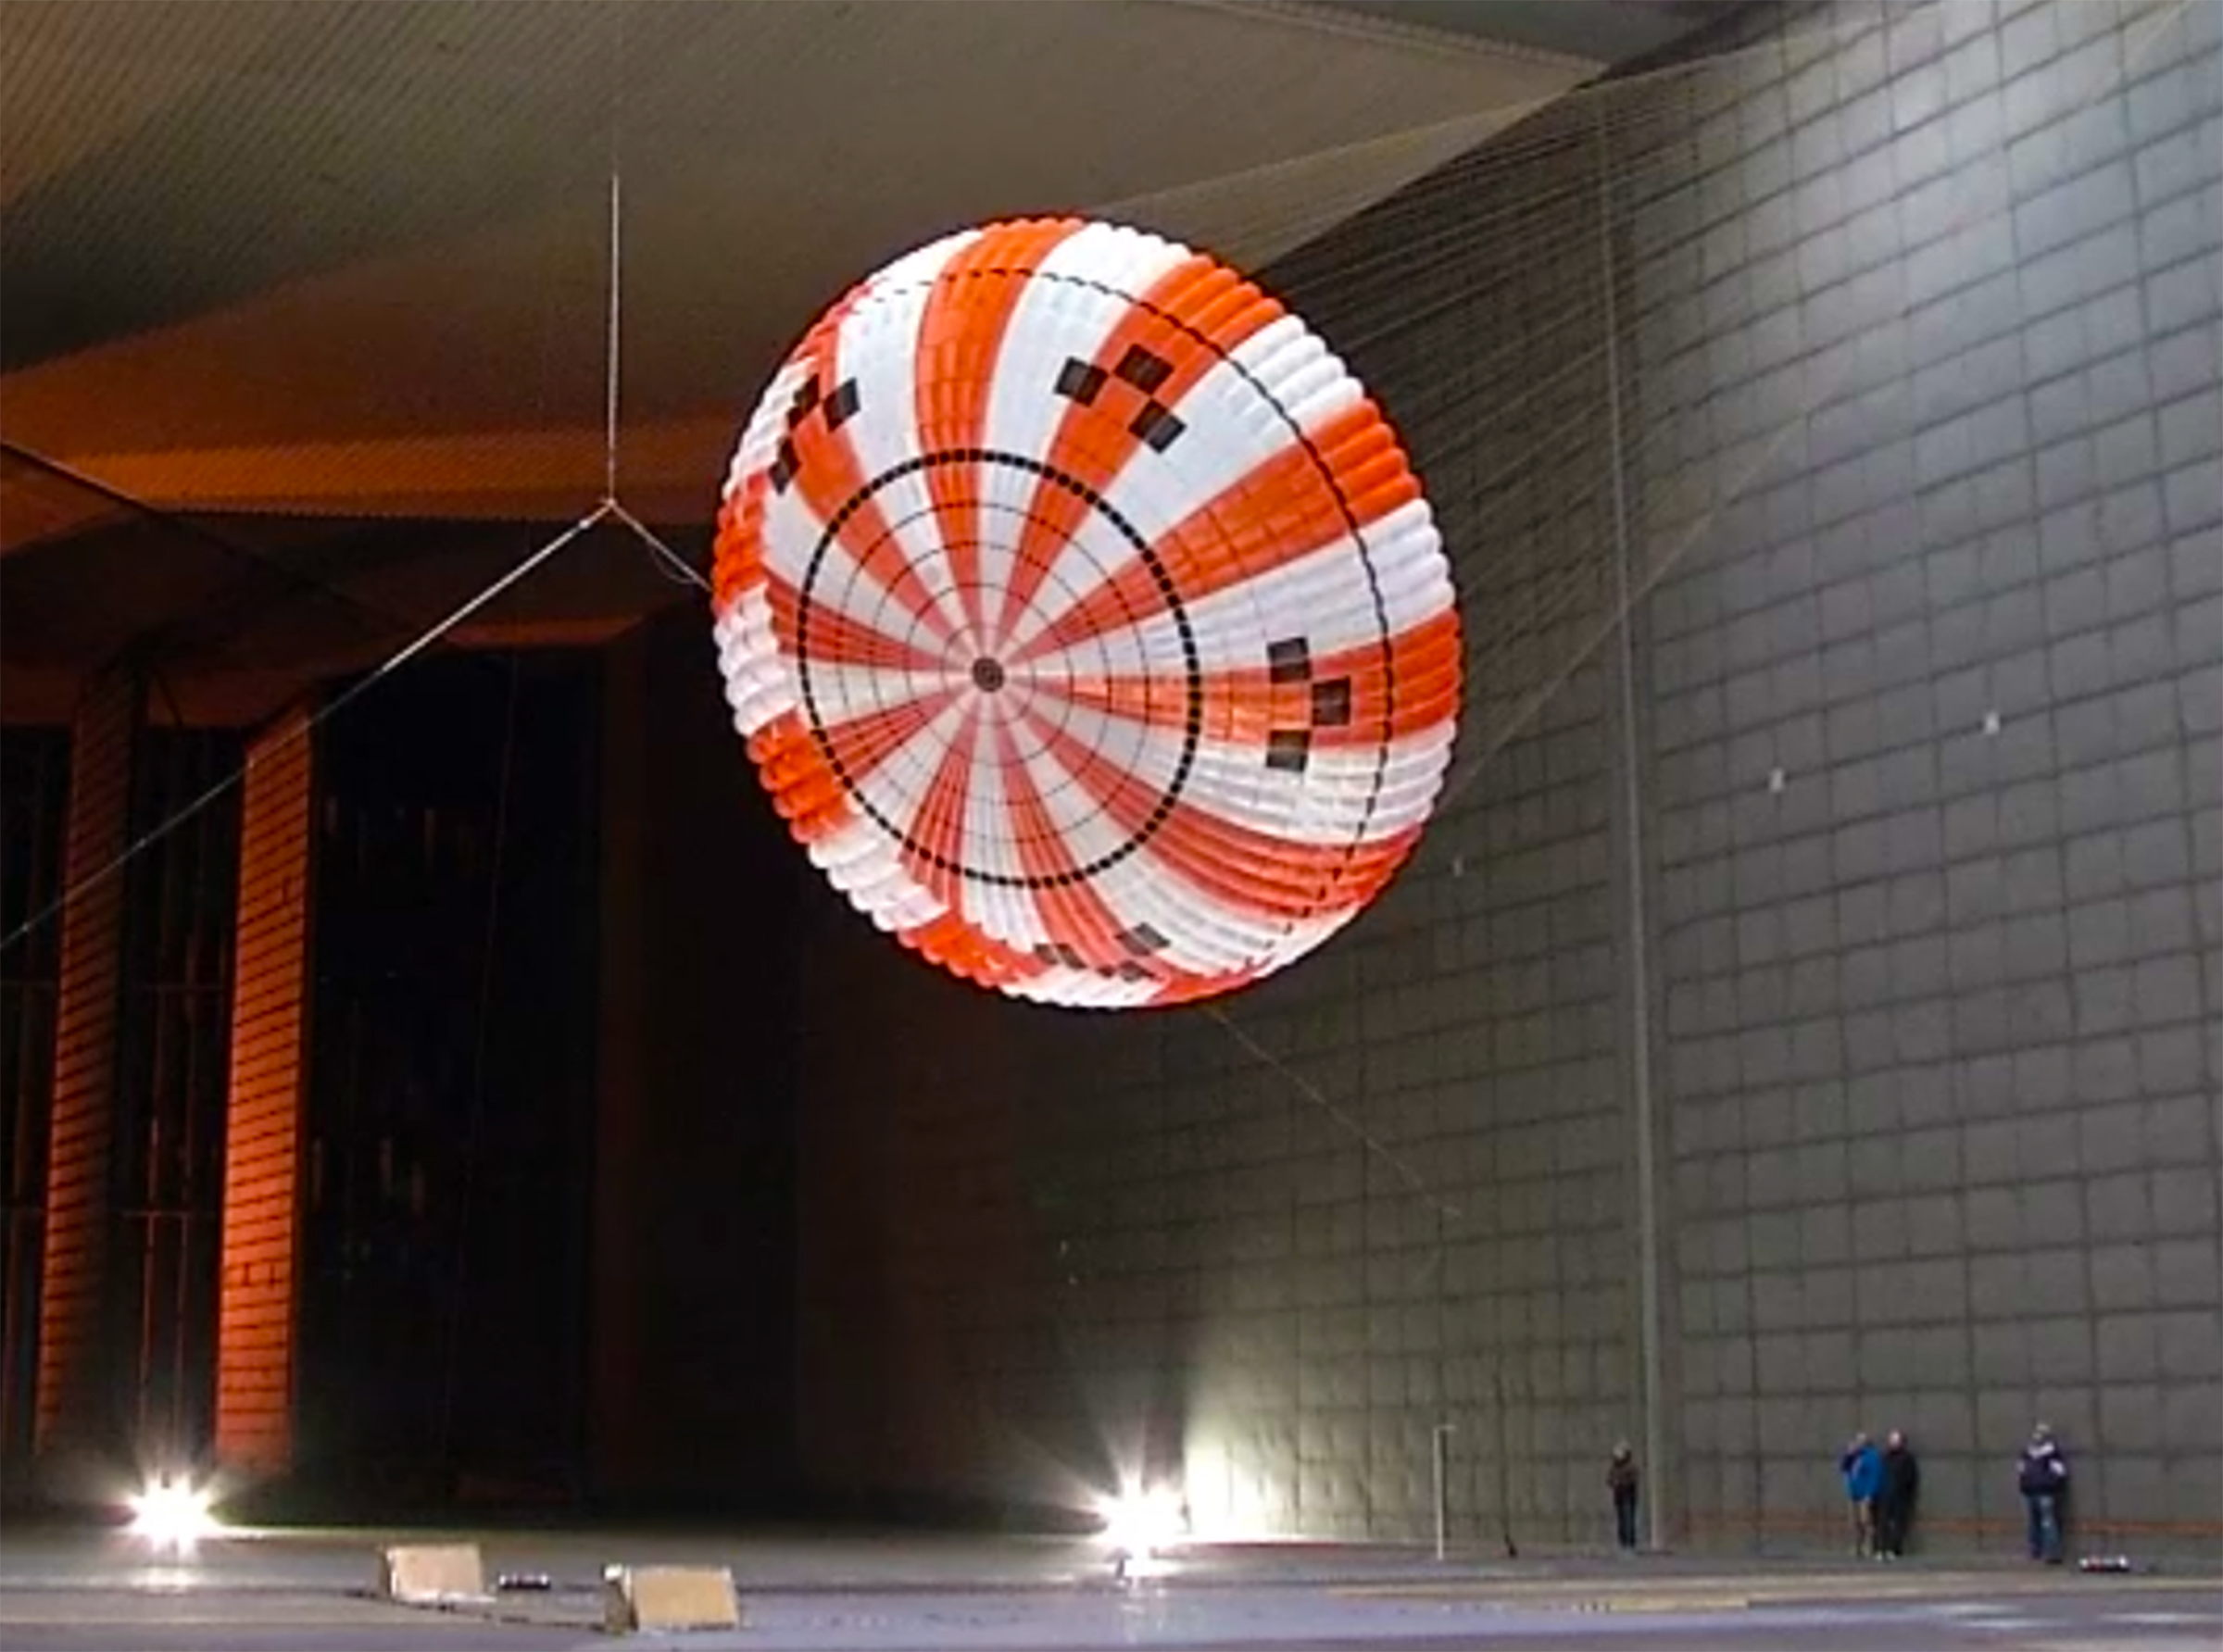
\includegraphics[width=0.45\textwidth]{Images/NFAC_OrionChute.jpg}
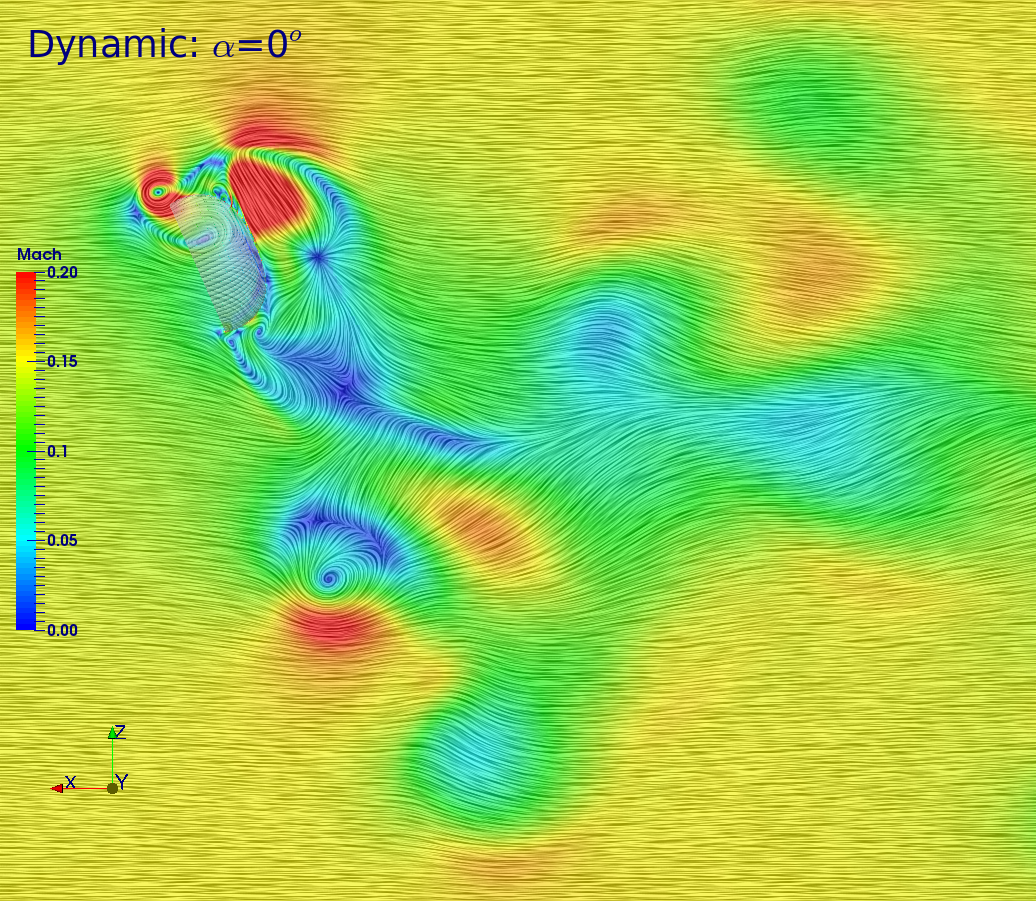
\includegraphics[width=0.45\textwidth]{Images/FlowVizDynamic.png}
\caption{Left: 1/3-scale wind tunnel test of Orion parachute.  Right: CFD solution of flow over a rigid parachute exhibiting pendulum motion}
\label{WTTandCFD}
\end{center}
\end{figure}
\vspace{-2em}


However, pendulum motion is a result of rate-dependent, dynamic forces, and it was of interest to the author to investigate the effect of relative motion of the parachute on the CFD results.  For this purpose, a moving geometry CFD simulation was developed, where the existing grid systems were modified to allow pendulum motion according to a prescribed equation during the simulation.

To validate the dynamic force simulation capability of the moving CFD model, results were compared to recent tests of a one-third scale Engineering Design Unit (EDU) geometry parachute in the National Full-scale Aerodynamic Complex (NFAC) 80x120 wind tunnel.  In this test, the parachute was secured by its risers upstream of the parachute, and maneuvered by tethers attached to the aft vent.  For the dynamic tests, the parachute was released at the vent an allowed to precess about the test section of the wind tunnel.  Load forces on the risers were recorded, allowing the direct calculation of aerodynamic coefficients for comparison with dynamic CFD results.\cite{blockage}


%%%%%%%%%%%%%%%%%%%%%%%%%%%%%%%%%%
\subsection{Turbulence Study Goals}

The CFD simulations described in the previous section employ an industry-standard RANS turbulence model that has proven to be effective similar, past studies, but the dependence of these solutions on the chosen turbulence model has never been investigated.  The focus of the analysis in this paper is a comparison of two RANS turbulence models applied to a simplified test case of the complex grid system described above.

A simplified, hemispherical shell grid was developed for this test to reduce the computational requirements, as the previously described simulations can take up to a week to run on hundreds of processors.  The motivation of this turbulence study was to demonstrate a general independence of the CFD solution from the chosen RANS model.

%%%%%%%%%%%%%%%%%%%%%%%%%%%%%%%%%%%%%%%%%%%%%%%%%%%%%%%%%%%%%%%%%%%%%%%%
\section{Turbulence Study Design}
%%%%%%%%%%%%%%%%%%%%%%%%%%%%%%%%%%%%%%%%%%%%%%%%%%%%%%%%%%%%%%%%%%%%%%%%


%%%%%%%%%%%%%%%%%%%%%%%%%%%%%%%%%%
\subsection{Solver Background}

CFD simulations were performed using OVERFLOW, an implicit Navier-Stokes solver, which employs finite-differencing methods on structured, overset grids.\cite{overflow}  Many solution algorithms and schemes are available, including Lower Upper-Symmetric Gauss Sidel (LU-SGS) implicit solution algorithm and implicit unfactored Successive Symmetric Over Relaxation SSOR algorithm.  Solution scheme and algorithm is chosen to appropriately compliment the chosen turbulence model and desired solution accuracy order.  OVERFLOW provides various turbulence models for use ranging from basic algebraic models to RANS methods to Large Eddy Simulation (LES).  Those used in this study will be detailed in the next section.

Dual-time stepping is also employed to aid in solution convergence.\cite{dualtime}  This process allows the solver to iterate on a steady solution between each physical time step.  This aids in pre-conditioning the unsteady solution for low Mach number cases.

OVERFLOW allows for the solution of multiple species gas continuity equations to aid in the solution of chemically reactive or high Mach flows.  For non-reactive flows, such as the one described in this paper, the fluid medium is treated as a single species, constant specific heat $\gamma$ gas.

One major advantage of OVERFLOW's structure, overset grid nature, is that relative grid motion can be achieved without extreme additional cost as it only requires calculating new grid interpolation schemes. \cite{gmp}  The Geometry Manipulation Protocol (GMP) allows the user to input prescribed motion equations or let the grids react freely to aerodynamic forces according to basic equations of motion.  It is for this capability that the author has selected this solver for this and the previous related study.


%%%%%%%%%%%%%%%%%%%%%%%%%%%%%%%%%%
\subsection{Turbulence Models}

This turbulence study concerns two RANS modeling methods: the Spalart-Almaras (SA) and Shear-Stress Transport (SST) models.  The SA model is a one-equation turbulence model that solves a single transport equation for a viscosity-related variable (e.g. Turbulent Kinetic Energy (TKE)).\cite{SAmodel} In OVERFLOW, it is solved using a second-order accurate Backward Differentiation Formula (BDF2) algorithm.

The SST model is a two-equation turbulence model that expands on the SA model by solving both a convection equation accounting for the energy of the turbulence and a dissipation equation accounting for the scale of the turbulence. \cite{menter_sst}  The SST model combines the features of other two-equation models, using the $k-\omega$ method for inner boundary layer solutions and the $k-\epsilon$ for freestream regions.


%%%%%%%%%%%%%%%%%%%%%%%%%%%%%%%%%%
\subsection{Case Parameters And Solution Process}

The CFD case discussed in this paper was solved at the same conditions as the high-fidelity parachute simulation, which has the geometry scale as the flight parachute but a velocity scaled up by a factor of five to aid in convergence at low Mach number.  The flight Reynolds number $Re$ is preserved by scaling down the density of the fluid medium.  Flow simulations are three-dimensional as this grid will ultimately be used for six degree-of-freedom moving-mesh simulations.

\begin{table}[htb]
\begin{center}
\begin{tabular}{| l | l | l |}
\hline
\textbf{Parameter} &  \textbf{Simulation Value} & \textbf{Notes} \\
\hline
Mach Number   &  $M=0.15$ ($V=1988in/s$) & Scaled up from flight      \\
Density &  $\rho=2.61x10^{-7}slug/in^3$ & Scaled down to preserve Re       \\
Temperature  &  $T=508^oR$ & Yields: $\mu=3.07x10^{-8}slug/in\cdot s$ \\
Reynolds Number  &  $Re/in=\frac{\rho V}{\mu}=16965/in$ & Full: $Re=2.36e7$\\
Reference Length  &  $L_{ref}=1392in$ & Parachute Diameter \\
Turbulence Models  &  SST, SA           & NQT=205, 102 \\
\hline
\end{tabular}
\end{center}
\caption{CFD simulation run parameters}
\end{table}

Simulations were converged according to a three-stage process.  Seeking a faster convergence than previous parachute simulations, all solution stages were time-accurate with Newton dual-time stepping from the beginning (as opposed to first converging as steady-state solution).  The nondimensional physical time step size $DTPHYS$ and number of Newton subiterations $NITNWT$ for each solver stage were as follows:

\begin{table}[htb]
\begin{center}
\begin{tabular}{| l | c | c |}
\hline
\textbf{Stage} &  \textbf{DTPHYS} & \textbf{NITNWT} \\
\hline
INPUT,1   &  0.25 & 5      \\
INPUT,2   &  10 & 15      \\
INPUT,3   &  2 & 5      \\
\hline
\end{tabular}
\end{center}
\caption{CFD simulation convergence parameters}
\end{table}

The first input stage was preceded by a full multi-grid process where an initial solution was converged on an extra-coarse grid.



%%%%%%%%%%%%%%%%%%%%%%%%%%%%%%%%%%
\subsection{Grid Design}

The computational mesh was designed to maintain the primary features of the original, high-fidelity parachute model in a much simpler representation so that diagnostic simulations such as those described in this paper can be performed quickly and numerously.  The same reference length was preserved from the original grid, but the parachute vent and gaps were eliminated due to their meshing complexity.  The mesh was also coarsened significantly to improve convergence time, resulting in 3062742 total grid points.


%%\vspace{-2em}
\begin{figure}[htb!]
\begin{center}
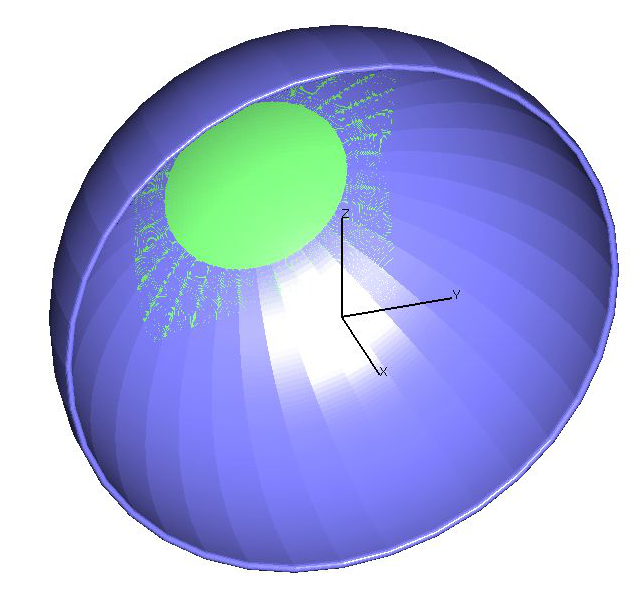
\includegraphics[width=0.45\textwidth]{Images/grid_surf.png}
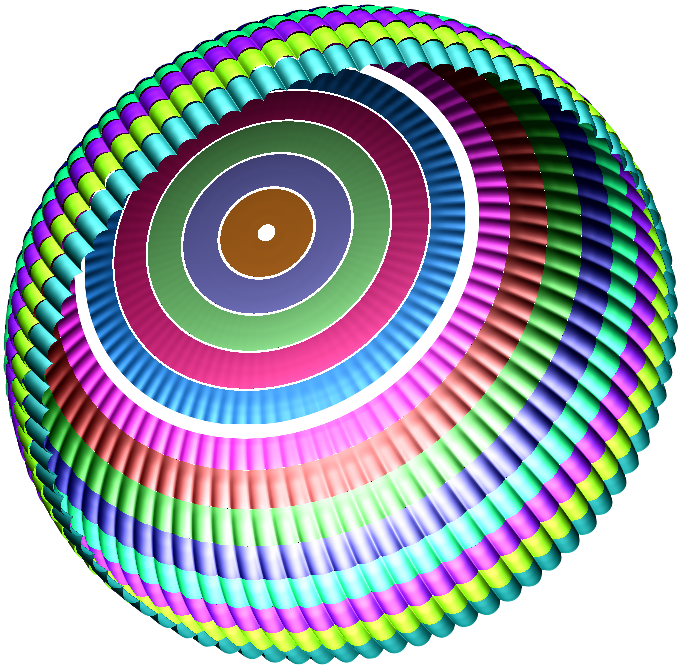
\includegraphics[width=0.45\textwidth]{Images/MPCV_chute_surf.png}
\caption{Left: Simple hemispherical shell grid ($3e6$ points).  Right: High-fidelity Orion MPCV parachute grid ($2e9$ points)}
\label{ChuteSurf}
\end{center}
\end{figure}
%%\vspace{-2em}


The overset grid structure of the original parachute simulation was emulated as well, with multiple, cascading box grids to propagate the flow around the parachute, and one dense box grid immediately surrounding the parachute to compensate for the near-body volume grids that were inadequately small due to the concave nature of the hemisphere's shape.


%%\vspace{-2em}
\begin{figure}[htb!]
\begin{center}
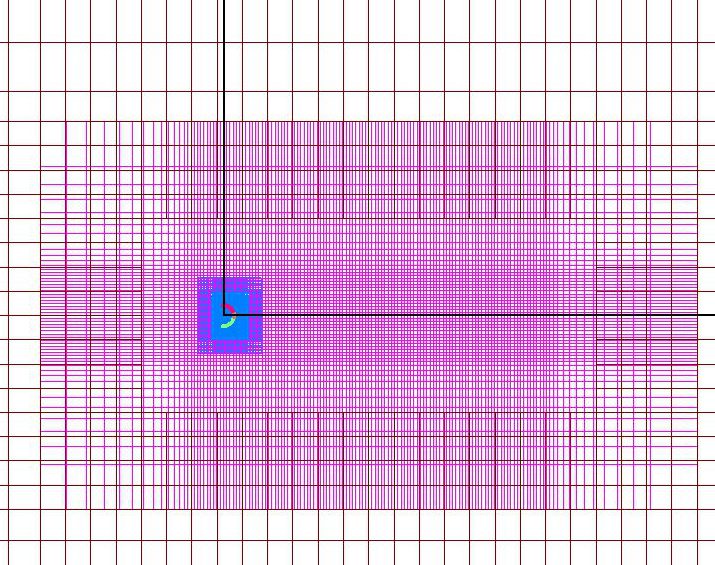
\includegraphics[width=0.45\textwidth]{Images/grid_wake.png}
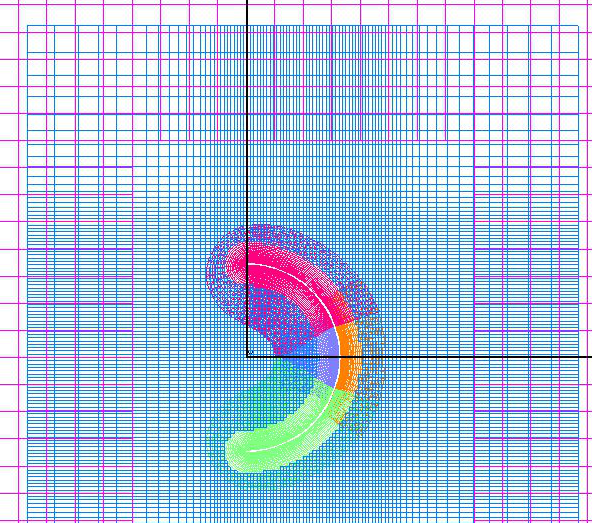
\includegraphics[width=0.45\textwidth]{Images/grid_body.png}
\caption{Left: Off-body box grid for freestream flow around hemispherical shell.  Right: Hemispherical shell body grid}
\label{BoxGrids}
\end{center}
\end{figure}
%%\vspace{-2em}


%%%%%%%%%%%%%%%%%%%%%%%%%%%%%%%%%%%%%%%%%%%%%%%%%%%%%%%%%%%%%%%%%%%%%%%%
\section{Results}
%%%%%%%%%%%%%%%%%%%%%%%%%%%%%%%%%%%%%%%%%%%%%%%%%%%%%%%%%%%%%%%%%%%%%%%%

In order to compare the differences of the two turbulence models, multiple analyses techniques were employed.  First, the convergence history of various force and moment coefficients was observed, as per Fig~\ref{ConvergHist}.

%%\vspace{-2em}
\begin{figure}[htb!]
\begin{center}
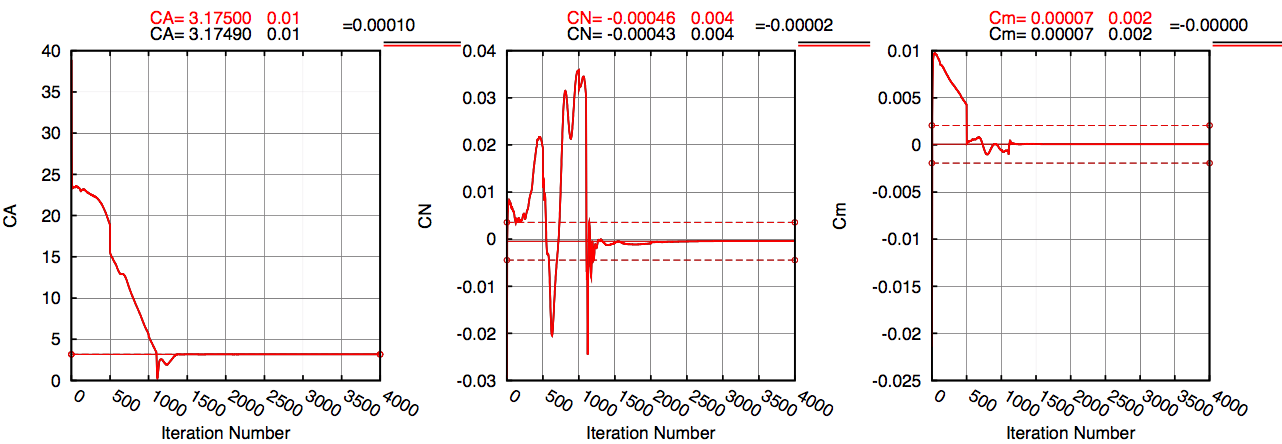
\includegraphics[width=\textwidth]{Images/ConvergHist.png}
\caption{Convergence history of both turbulence models showing perfect overlap (From left to right, coefficients of: axial force, normal force, and pitching moment)}
\label{ConvergHist}
\end{center}
\end{figure}
\vspace{-2em}

The figure makes it obvious that there is practically no difference in the convergence histories of the two simulations.  Interestingly, the change from Inputs deck 2 to 3 (at iteration 2000) shows no obvious change, despite a quartering of the physical time step.  This suggests that the solution of this problem is somewhat independent of the chosen turbulence model but also indicate that there may be other factors of dependence, such as grid spacing.

Investigating the flow visually reveals some of these grid dependencies.  The left image in Fig~\ref{FlowVizClose} demonstrates obviously contrasting regions within the grid.  This is due to overlapping grid of different coarsenesses, as shown in the right image.

%%\vspace{-2em}
\begin{figure}[htb!]
\begin{center}
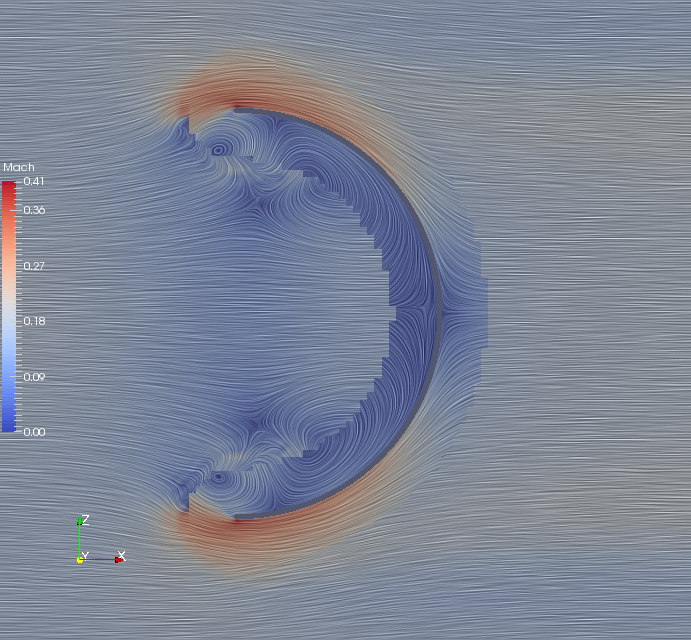
\includegraphics[width=0.45\textwidth]{Images/sst_mach_lic.png}
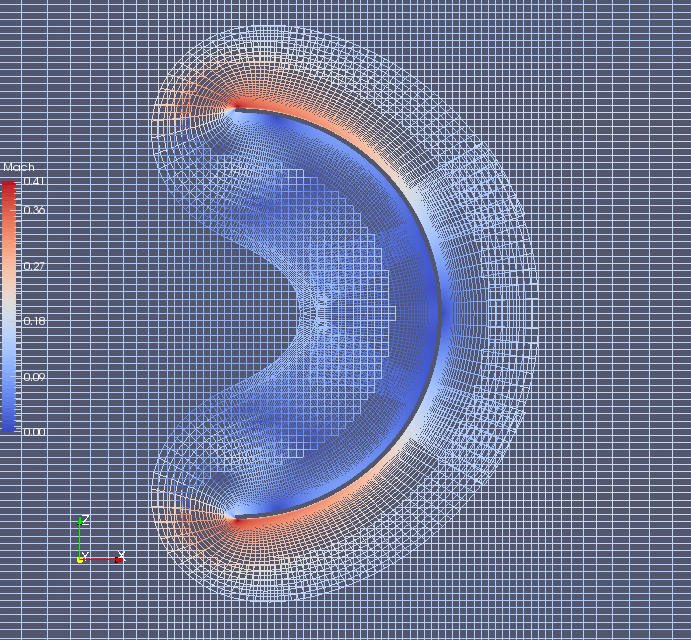
\includegraphics[width=0.45\textwidth]{Images/sst_mach_wire.png}
\caption{Flow Mach number visualization of SST turbulence model results (SA flow essentially identical) Left: Mach contours and streamlines.  Right: Mach values at grid points}
\label{FlowVizClose}
\end{center}
\end{figure}
%%\vspace{-2em}



Due to the highly coarse nature of this experimental grid, interpolation between grids is unideal in some locations, causing grid-dependency within the solution.  Most obviously, the flow very near the hemisphere is ``captured'' in the very fine near-body volume grid.  Eddies are well defined in this region, but are discontinuous and less resolved when crossing into other grids.

Though these plots demonstrate that this grid and solution are not extremely well-conditions for production CFD, they may still serve a purpose as a turbulence model testbed.  This flow was further analyzed by observing the wake x-velocity profiles created by this hemispherical body, sampled from the lines indicated below in Fig~\ref{SampleLines}.

%%\vspace{-2em}
\begin{figure}[htb!]
\begin{center}
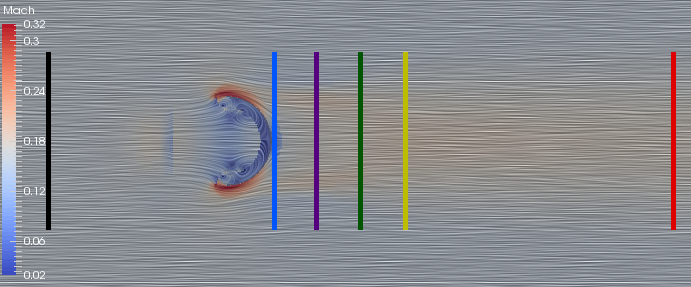
\includegraphics[width=\textwidth]{Images/SampleLines_color.png}
\caption{Wake velocity profile sampling lines}
\label{SampleLines}
\end{center}
\end{figure}
%%\vspace{-2em}

Aside from the sample locations, the above figure also reveals another flow feature indicating grid dependence: the linear flow distortion directly in front of the hemisphere caused by grid interpolation.

%%\vspace{-2em}
\begin{figure}[htb!]
\begin{center}
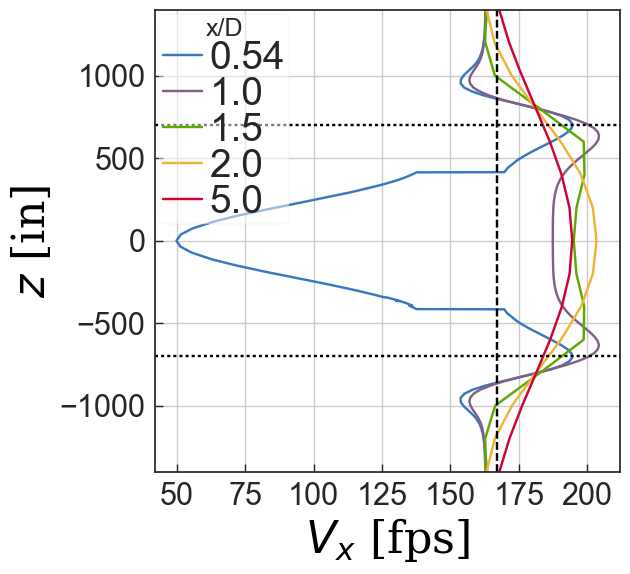
\includegraphics[width=0.45\textwidth]{Images/wakelines_sst_Vx.png}
\caption{Wake velocity profiles sampled at various streamwise locations for the SST simulation (Vertical dashed line is freestream velocity profile, horizontal dotted lines are edges of hemisphere geometry)}
\label{WakeProfiles}
\end{center}
\end{figure}
%%\vspace{-2em}

The plot at the end of the document in Fig~\ref{WakeProfilesBoth} shows that at every streamwise station, both turbulence models have identical results.  Further analysis of the difference of these two solutions demonstrated that the only difference was due to floating point error and grid discontinuities.  The image on the right shows wake velocity results for only one case.  These exhibit the expected behavior of flow behind a bluff body, ranging from the most distorted just behind the hemisphere geometry and approaching the freestream distribution further downstream.

Finally, the integral effect of velocity distribution can be measured by integrating the momentum deficit to obtain a drag coefficient.  For this computational simulation, the drag coefficient was computed to be $C_D=3.2$, which is significantly higher than experimental values for a semicircle $C_D=2.3$.  Some reasonable causes for this discrepancy could be the difference between 2D and 3D flow and the general inaccuracy of RANS in modeling massively separated flow, but this result combined with the other previous observations suggests strongly that grid refinement will yield a different solution.

%%%%%%%%%%%%%%%%%%%%%%%%%%%%%%%%%%%%%%%%%%%%%%%%%%%%%%%%%%%%%%%%%%%%%%%%
\section{Conclusions and Future Work}
%%%%%%%%%%%%%%%%%%%%%%%%%%%%%%%%%%%%%%%%%%%%%%%%%%%%%%%%%%%%%%%%%%%%%%%%

The results of this turbulence modeling comparison could suggest that the RANS simulation of flow over a parachute-like body is somewhat independent of turbulence model choice, but further testing is required to make this assertion definitively.  Further refinement of the grid may yield turbulent effects that are not observed in this coarse simulation.

This grid system will be utilized in the future as a test bed for 6-DoF pendulum motion simulations.  This should serve as an avenue for further testing of the effect of turbulence modeling.



%%%%%%%%%%%%%%%%%%%%%%%%%%%%%%%%%%%%%%%%%%%%%%%%%%%%%%%%%%%%%%%%%%%%%%%%
\begin{thebibliography}{9}% maximum number of references (for label width)
%%%%%%%%%%%%%%%%%%%%%%%%%%%%%%%%%%%%%%%%%%%%%%%%%%%%%%%%%%%%%%%%%%%%%%%%

 \bibitem{ray:15}
 E. S. Ray and R. A. Machin, ``Pendulum Motion in Main Parachute Clusters,'' in {\it 23rd AIAA Aerodynamic Decelerator Systems Technology Conference}, Submitted, 2015.

 \bibitem{menter_sst}
 F. R. Menter and Christopher L. Rumsey, ``Assessment of Two-Equation Turbulence Models for Transonic Flows,'' in {\it 25th AIAA Fluid Dynamics Conference}, Submitted, 1994.

 \bibitem{schwing15}
 J. S. Greathouse and A. M. Schwing, ``Study of Geometric Porosity on Static Stability and Drag using Computational Fluid Dynamics for Rigid Parachute Shapes,'' in {\it 23rd AIAA Aerodynamic Decelerator Systems Technology Conference}, Submitted, 2015.

 \bibitem{overflow}
 R. H. Nichols, R. W. Tramel, and P. G. Buning, “Solver and Turbulence Model Upgrades to OVERFLOW 2 for Unsteady and High-Speed Applications,” No. AIAA 2006-2824, 2006.

 \bibitem{gmp}
 S. M. Murman, W. M. Chan, M. J. Aftosmis, and R. L. Meakin, ``An Interface for Specifying Rigid-Body Motions for CFD Applications,'' AIAA Paper 2003-1237, 2003.

 \bibitem{blockage}
 J. M. Macha and R. J. Buffington, ``Wall-Interference Corrections for Parachutes in a Closed Wind Tunnel,'' {\it Journal of Aircraft}, Vol. 27, No. 4, pp. 320-325, April 1990.

\bibitem{dualtime}
Pandya, S. A., Venkateswaran, S., and Pulliam, T. H., “Implementation of Preconditioned Dual-Time Procedures in
OVERFLOW”, AIAA-2003-0072, Jan. 2003.

\bibitem{SAmodel}
P. R. Spalart and S. R. Allmaras., "A One-Equation Turbulence Model for Aerodynamic Flows", AIAA-92-0439, January 1992.

 % \bibitem{wtt}
 % nfac test report?

\end{thebibliography}

%%\vspace{-2em}
\begin{figure}[htb]
\begin{center}
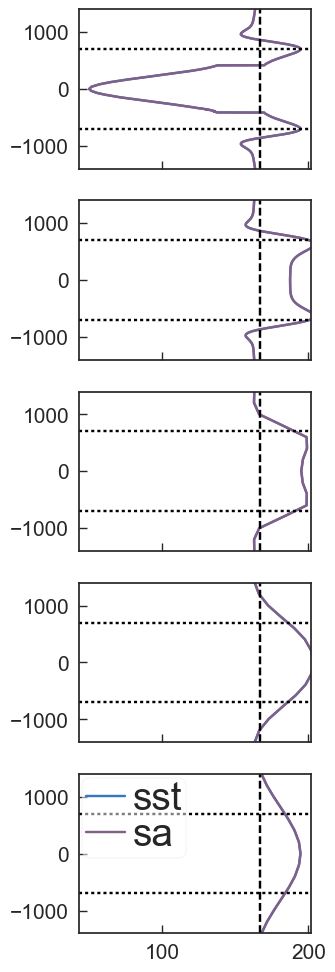
\includegraphics[width=0.45\textwidth]{Images/wakelines_all_Vx.png}
\caption{Wake velocity profiles sampled at various streamwise locations showing identical overlap of SST and SA turbulence models}
\label{WakeProfilesBoth}
\end{center}
\end{figure}





\end{document}


